\ifx\wholebook\relax\else

% --------------------------------------------
% Lulu:

    \documentclass[a4paper,12pt,twoside]{../includes/ThesisStyle}

	\usepackage[T1]{fontenc} %%%key to get copy and paste for the code!
%\usepackage[utf8]{inputenc} %%% to support copy and paste with accents for frnehc stuff
\usepackage{times}
\usepackage{ifthen}
\usepackage{xspace}
\usepackage{alltt}
\usepackage{latexsym}
\usepackage{url}            
\usepackage{amssymb}
\usepackage{amsfonts}
\usepackage{amsmath}
\usepackage{stmaryrd}
\usepackage{enumerate}
\usepackage{cite}
%\usepackage[pdftex,colorlinks=true,pdfstartview=FitV,linkcolor=blue,citecolor=blue,urlcolor=blue]{hyperref}
\usepackage{xspace}
%\usepackage{graphicx}
\usepackage{subfigure}
\usepackage[scaled=0.85]{helvet}
        
        
\newcommand{\sepe}{\mbox{>>}}
\newcommand{\pack}[1]{\emph{#1}}
\newcommand{\ozo}{\textsc{oZone}\xspace}
\newcommand\currentissues{\par\smallskip\textbf{Current Issues -- }}

\newboolean{showcomments}
\setboolean{showcomments}{true}
\ifthenelse{\boolean{showcomments}}
  {\newcommand{\bnote}[2]{
	\fbox{\bfseries\sffamily\scriptsize#1}
    {\sf\small$\blacktriangleright$\textit{#2}$\blacktriangleleft$}
    % \marginpar{\fbox{\bfseries\sffamily#1}}
   }
   \newcommand{\cvsversion}{\emph{\scriptsize$-$Id: macros.tex,v 1.1.1.1 2007/02/28 13:43:36 bergel Exp $-$}}
  }
  {\newcommand{\bnote}[2]{}
   \newcommand{\cvsversion}{}
  } 


\newcommand{\here}{\bnote{***}{CONTINUE HERE}}
\newcommand{\nb}[1]{\bnote{NB}{#1}}
\newcommand{\fix}[1]{\bnote{FIX}{#1}}
%%%% add your own macros 

\newcommand{\sd}[1]{\bnote{Stef}{#1}}
\newcommand{\ja}[1]{\bnote{Jannik}{#1}}
\newcommand{\na}[1]{\bnote{Nico}{#1}}
%%% 


\newcommand{\figref}[1]{Figure~\ref{fig:#1}}
\newcommand{\figlabel}[1]{\label{fig:#1}}
\newcommand{\tabref}[1]{Table~\ref{tab:#1}}
\newcommand{\layout}[1]{#1}
\newcommand{\commented}[1]{}
\newcommand{\secref}[1]{Section \ref{sec:#1}}
\newcommand{\seclabel}[1]{\label{sec:#1}}

%\newcommand{\ct}[1]{\textsf{#1}}
\newcommand{\stCode}[1]{\textsf{#1}}
\newcommand{\stMethod}[1]{\textsf{#1}}
\newcommand{\sep}{\texttt{>>}\xspace}
\newcommand{\stAssoc}{\texttt{->}\xspace}

\newcommand{\stBar}{$\mid$}
\newcommand{\stSelector}{$\gg$}
\newcommand{\ret}{\^{}}
\newcommand{\msup}{$>$}
%\newcommand{\ret}{$\uparrow$\xspace}

\newcommand{\myparagraph}[1]{\noindent\textbf{#1.}}
\newcommand{\eg}{\emph{e.g.,}\xspace}
\newcommand{\ie}{\emph{i.e.,}\xspace}
\newcommand{\ct}[1]{{\textsf{#1}}\xspace}


\newenvironment{code}
    {\begin{alltt}\sffamily}
    {\end{alltt}\normalsize}

\newcommand{\defaultScale}{0.55}
\newcommand{\pic}[3]{
   \begin{figure}[h]
   \begin{center}
   \includegraphics[scale=\defaultScale]{#1}
   \caption{#2}
   \label{#3}
   \end{center}
   \end{figure}
}

\newcommand{\twocolumnpic}[3]{
   \begin{figure*}[!ht]
   \begin{center}
   \includegraphics[scale=\defaultScale]{#1}
   \caption{#2}
   \label{#3}
   \end{center}
   \end{figure*}}

\newcommand{\infe}{$<$}
\newcommand{\supe}{$\rightarrow$\xspace}
\newcommand{\di}{$\gg$\xspace}
\newcommand{\adhoc}{\textit{ad-hoc}\xspace}

\usepackage{url}            
\makeatletter
\def\url@leostyle{%
  \@ifundefined{selectfont}{\def\UrlFont{\sf}}{\def\UrlFont{\small\sffamily}}}
\makeatother
% Now actually use the newly defined style.
\urlstyle{leo}



	\usepackage{amsmath,amssymb}             % AMS Math
% \usepackage[french]{babel}
\usepackage[latin1]{inputenc}
\usepackage[T1]{fontenc}
\usepackage[left=1.5in,right=1.3in,top=1.1in,bottom=1.1in,includefoot,includehead,headheight=13.6pt]{geometry}
\renewcommand{\baselinestretch}{1.05}

\usepackage{multicol}

% Table of contents for each chapter

\usepackage[nottoc, notlof, notlot]{tocbibind}
\usepackage{minitoc}
\setcounter{minitocdepth}{1}
\mtcindent=15pt
% Use \minitoc where to put a table of contents

\usepackage{enumitem}

\usepackage{aecompl}

% Glossary / list of abbreviations

%\usepackage[intoc]{nomencl}
%\renewcommand{\nomname}{List of Abbreviations}
%
%\makenomenclature

% My pdf code

\usepackage[pdftex]{graphicx}
\usepackage[a4paper,pagebackref,hyperindex=true]{hyperref}

\usepackage{pgfplotstable,booktabs,colortbl}
\pgfplotsset{compat=1.8}

% Links in pdf
\usepackage{color}
\definecolor{linkcol}{rgb}{0,0,0.4} 
\definecolor{citecol}{rgb}{0.5,0,0} 

% Change this to change the informations included in the pdf file

% See hyperref documentation for information on those parameters

\hypersetup
{
bookmarksopen=true,
pdftitle="Sista: a Metacircular Architecture for Runtime Optimisation Persistence",
pdfauthor="Clement BERA", 
pdfsubject="Thesis", %subject of the document
%pdftoolbar=false, % toolbar hidden
pdfmenubar=true, %menubar shown
pdfhighlight=/O, %effect of clicking on a link
colorlinks=true, %couleurs sur les liens hypertextes
pdfpagemode=None, %aucun mode de page
pdfpagelayout=SinglePage, %ouverture en simple page
pdffitwindow=true, %pages ouvertes entierement dans toute la fenetre
linkcolor=linkcol, %couleur des liens hypertextes internes
citecolor=citecol, %couleur des liens pour les citations
urlcolor=linkcol %couleur des liens pour les url
}

% definitions.
% -------------------

\setcounter{secnumdepth}{3}
\setcounter{tocdepth}{1}

% Some useful commands and shortcut for maths:  partial derivative and stuff

\newcommand{\pd}[2]{\frac{\partial #1}{\partial #2}}
\def\abs{\operatorname{abs}}
\def\argmax{\operatornamewithlimits{arg\,max}}
\def\argmin{\operatornamewithlimits{arg\,min}}
\def\diag{\operatorname{Diag}}
\newcommand{\eqRef}[1]{(\ref{#1})}

\usepackage{rotating}                    % Sideways of figures & tables
%\usepackage{bibunits}
%\usepackage[sectionbib]{chapterbib}          % Cross-reference package (Natural BiB)
%\usepackage{natbib}                  % Put References at the end of each chapter
                                         % Do not put 'sectionbib' option here.
                                         % Sectionbib option in 'natbib' will do.
\usepackage{fancyhdr}                    % Fancy Header and Footer

% \usepackage{txfonts}                     % Public Times New Roman text & math font
  
%%% Fancy Header %%%%%%%%%%%%%%%%%%%%%%%%%%%%%%%%%%%%%%%%%%%%%%%%%%%%%%%%%%%%%%%%%%
% Fancy Header Style Options

\pagestyle{fancy}                       % Sets fancy header and footer
\fancyfoot{}                            % Delete current footer settings

%\renewcommand{\chaptermark}[1]{         % Lower Case Chapter marker style
%  \markboth{\chaptername\ \thechapter.\ #1}}{}} %

%\renewcommand{\sectionmark}[1]{         % Lower case Section marker style
%  \markright{\thesection.\ #1}}         %

\fancyhead[LE,RO]{\bfseries\thepage}    % Page number (boldface) in left on even
% pages and right on odd pages
\fancyhead[RE]{\bfseries\nouppercase{\leftmark}}      % Chapter in the right on even pages
\fancyhead[LO]{\bfseries\nouppercase{\rightmark}}     % Section in the left on odd pages

\let\headruleORIG\headrule
\renewcommand{\headrule}{\color{black} \headruleORIG}
\renewcommand{\headrulewidth}{1.0pt}
\usepackage{colortbl}
\arrayrulecolor{black}

\fancypagestyle{plain}{
  \fancyhead{}
  \fancyfoot{}
  \renewcommand{\headrulewidth}{0pt}
}

\usepackage{algorithm}
\usepackage[noend]{algorithmic}

%%% Clear Header %%%%%%%%%%%%%%%%%%%%%%%%%%%%%%%%%%%%%%%%%%%%%%%%%%%%%%%%%%%%%%%%%%
% Clear Header Style on the Last Empty Odd pages
\makeatletter

\def\cleardoublepage{\clearpage\if@twoside \ifodd\c@page\else%
  \hbox{}%
  \thispagestyle{empty}%              % Empty header styles
  \newpage%
  \if@twocolumn\hbox{}\newpage\fi\fi\fi}

\makeatother
 
%%%%%%%%%%%%%%%%%%%%%%%%%%%%%%%%%%%%%%%%%%%%%%%%%%%%%%%%%%%%%%%%%%%%%%%%%%%%%%% 
% Prints your review date and 'Draft Version' (From Josullvn, CS, CMU)
\newcommand{\reviewtimetoday}[2]{\special{!userdict begin
    /bop-hook{gsave 20 710 translate 45 rotate 0.8 setgray
      /Times-Roman findfont 12 scalefont setfont 0 0   moveto (#1) show
      0 -12 moveto (#2) show grestore}def end}}
% You can turn on or off this option.
% \reviewtimetoday{\today}{Draft Version}
%%%%%%%%%%%%%%%%%%%%%%%%%%%%%%%%%%%%%%%%%%%%%%%%%%%%%%%%%%%%%%%%%%%%%%%%%%%%%%% 

\newenvironment{maxime}[1]
{
\vspace*{0cm}
\hfill
\begin{minipage}{0.5\textwidth}%
%\rule[0.5ex]{\textwidth}{0.1mm}\\%
\hrulefill $\:$ {\bf #1}\\
%\vspace*{-0.25cm}
\it 
}%
{%

\hrulefill
\vspace*{0.5cm}%
\end{minipage}
}

\let\minitocORIG\minitoc
\renewcommand{\minitoc}{\minitocORIG \vspace{1.5em}}

\usepackage{multirow}
\usepackage{slashbox}

\newenvironment{bulletList}%
{ \begin{list}%
	{$\bullet$}%
	{\setlength{\labelwidth}{25pt}%
	 \setlength{\leftmargin}{30pt}%
	 \setlength{\itemsep}{\parsep}}}%
{ \end{list} }

\newtheorem{definition}{D�finition}
\renewcommand{\epsilon}{\varepsilon}

% centered page environment

\newenvironment{vcenterpage}
{\newpage\vspace*{\fill}\thispagestyle{empty}\renewcommand{\headrulewidth}{0pt}}
{\vspace*{\fill}}



	\graphicspath{{.}{../figures/}}
	\begin{document}
\fi

\chapter{Metacircular optimising JIT}
\label{chap:metacircular}
\minitoc

%Intro
By design, Scorch's optimiser and deoptimiser are written in Smalltalk and are running in the same runtime than the optimised application. This design leads to recursion problems similar to the ones existing in metacircular virtual machines, detailled in this Chapter. 

%single-threaded -> for comparison with Graal and co later
As Pharo is currently single-threaded, it is not possible to run Scorch in a concurrent native thread. To optimise code, Scorch requires either to temporarily interrupt the application green thread or to postpone the optimisation to a background-priority green thread as described in Section \ref{sec:optModes}. The deoptimiser cannot however postpone the deoptimisation of a frame as it would block completely the running application. The deoptimiser has necessarily to interrupt the application green thread to deoptimise the stack.

%introduction of the main issue
Hot spots can be detected in any Smalltalk code using conditionnal branches, including Scorch optimiser code itself (as Scorch is written in Smalltalk). When a hot spot is detected in the optimiser code, the optimiser interrupts itself and starts to optimise one of its own functions. While doing so, the same hot spot may be detected again before the optimised function is installed, leading the optimiser to interrupt itself repeatedly. This problem is discussed in Section \ref{sec:optRec}.

A similar problem exists for the deoptimiser. As the Scorch deoptimiser is written in Smalltalk, its code base may get optimised. One of the optimisation-time speculation may be incorrect at runtime, leading the deoptimiser to require the deoptimisation of one of its own frame. In this case, the deoptimiser calls itself on one of its own frame, which may require to deoptimise another frame for the same function, leading the deoptimiser to call itself repeatedly. This second problem is detailled in Section \ref{sec:deoptRec}.

We call the \emph{infinite recursion} problem this issue where the optimiser or the deoptimiser calls itself repeatedly.

%Different constraint so different solutions
The optimiser and deoptimiser have different constraints. It is possible to disable temporarily the optimiser while the application is running. In the worst case, a disabled optimiser leads some functions not to be optimised, but the application keeps running correctly. However, the deoptimiser cannot be disabled temporarily while the application is running as an application requiring deoptimisation cannot continue to execute code until the deoptimisation is performed. As the optimiser and the deoptimiser have different constraints, they need different solutions for the infinite recursion problem.

%Outline and solution
This chapter explains the design used to avoid the infinite recursion issue in both the optimiser and the deoptimiser. Section \ref{sec:optRec} describes how the problem is solved for the optimiser by temporarily disabling it in specific circumstances. Section \ref{sec:deoptRec} shows how the deoptimiser solves the problem by using a code base completely independent from the rest of the system that cannot be optimised, to never require to be deoptimised. Section \ref{sec:recRelW} discuss similar designs in other VMs and compares our solution to other solutions when relevant.

%%%%%%%%%%%%%%%%%%%%%%%%%%%%%%%%%%%%%%%%%%%%%%%%%%%%%%%%%%%%%%%%%%%%%%%%%%%%%%%%%%%%%%%%%%%%%%%%%%%%%%%%%%%%%%%%%%%%%%%%%%%%%

\section{Scorch optimiser}
\label{sec:optRec}

%Intro, what Scorch optimiser does and critical mode.
Scorch optimiser is activated by the VM when a hot spot is detected. As Pharo is single-threaded, the optimiser is activated by interrupting the application green thread. The optimiser chooses, based on the current stack, a v-function to optimise.  Once the v-function to optimise is chosen, the optimiser gets started in critical mode: it attempts to generate an optimised v-function in a limited time period. If it succeeds, the optimised v-function is installed and used by further calls on the function. If the optimiser fails to generate the optimised v-function in the limited time period, it adds the v-function to a background compilation queue. In any case, the application is then resumed. When the application becomes idle, if the background compilation queue is not empty, Scorch gets activated in background mode. It produces and installs optimised v-functions for each function in the compilation queue without any time limit. 

\subsection{Infinite recursion issue}

%repeat problem for optimiser
As Scorch optimiser is written in Smalltalk, it can theoretically optimise its own code. In practice, if it happens, it may lead to an infinite recursion. Indeed, each time Scorch tries to optimise a function, before reaching the point where it can install the optimised function, it may interrupt itself to start optimising one of its own function. If a hot spot is detected in the optimiser code each time it attempts to optimise anything, then the optimiser never reaches the point where it can install an optimised function.

Figure \ref{fig:InfiniteRecursionOptPb} shows the problem. On the left, in the normal optimisation flow, the application is interrupted when a hot spot is detected. The optimiser generates an optimised v-function, installs it and the application resumes. On the right, in the infinite recursion issue, the application is also interrupted when a hot spot is detected. While the optimiser is generating an optimised function, a hot spot is detected in the optimiser code. The optimiser then restarts to optimise one of its own functions, but another hot spot is detected in the optimiser code: the optimiser keeps restarting the optimisation of one of its own function.

\begin{figure}[h!]
    \begin{center}
        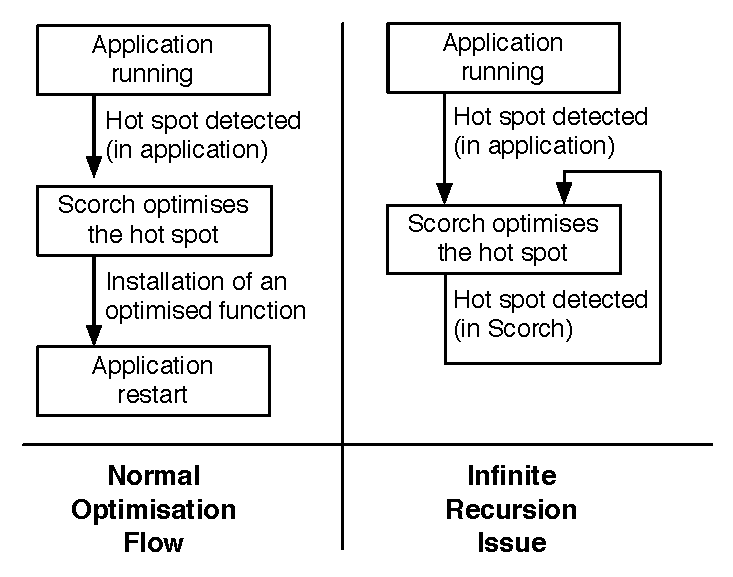
\includegraphics[width=0.65\linewidth]{InfiniteRecursionOptPb}
        \caption{Infinite recursion problem during optimisation}
        \label{fig:InfiniteRecursionOptPb}
    \end{center}
\end{figure}

This problem has different consequences depending if the optimiser is started in critical or in background mode. In practice, the infinite recursion issue leads to a massive performance loss.

%slow down - critical
\paragraph{Critical mode.} In critical mode, the optimiser has a limited time period to optimise code. If the infinite recursion issue happens, the optimiser spins until the time period ends as shown in Figure \ref{fig:InfiniteRecursionOptPbCritical}. The application is then resumed without any optimised function installed. The application gets drastically slower as it gets interrupted for the full critical mode time period without gaining any performance from those interruptions.

\begin{figure}[h!]
    \begin{center}
		\subfigure[Critical mode]{\label{fig:InfiniteRecursionOptPbCritical}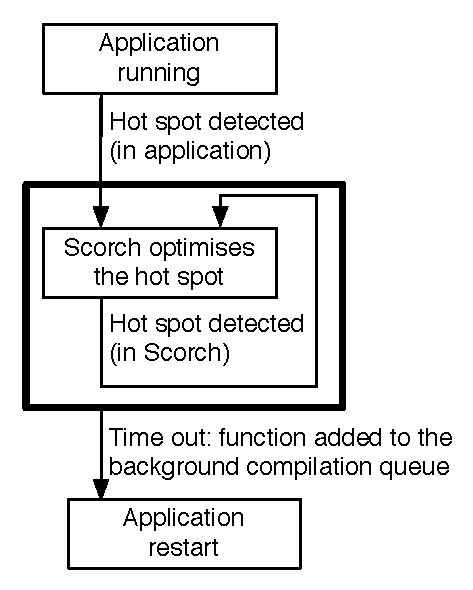
\includegraphics[width=0.3\linewidth]{InfiniteRecursionOptPbCritical}}
		\hspace{1cm}
		\subfigure[Background mode]{\label{fig:InfiniteRecursionOptPbBackground}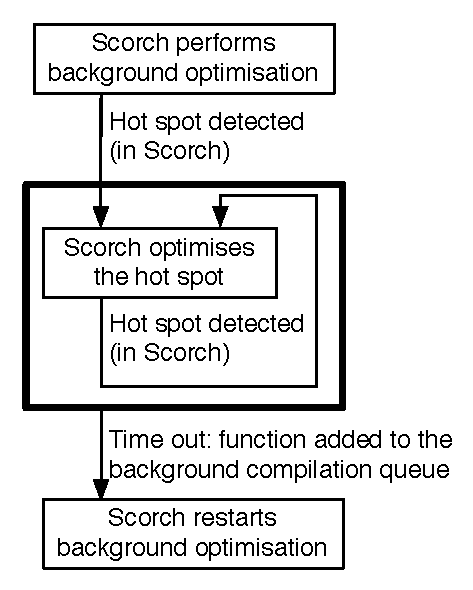
\includegraphics[width=0.3\linewidth]{InfiniteRecursionOptPbBackground}}
		
		\subfigure{
\includegraphics[width=0.3\linewidth]{InfiniteRecursionOptPbLegend}}
		\caption{Infinite recursion problem in the two optimisation modes}
    \end{center}
\end{figure}

%slow down - background
%It can conceptually happen that the optimiser starts spinning while searching the stack for a function to optimise. In this case, no function can be added to the background compilation queue as the optimiser has not been able to find a function to optimise in the limited time period. In practice, in our case, the stack search code is quite simple and in practice no hot spot can be detected repeatedly in this code.

\paragraph{Background mode.} When the application becomes idle, the optimiser is started in background mode to optimise functions in the background compilation queue. In this case, the optimiser always successfully generates and installs optimised functions. However, the optimisation of a function is very slow. Indeed, while the optimiser is running in background mode, it activates itself multiple times in critical mode when detecting hot spots in its own code. Each time it happens, the optimiser spins in critical mode for the time period allowed as shown on Figure \ref{fig:InfiniteRecursionOptPbBackground}. If the optimiser is started many times on itself during background optimisation, the optimisation of the function may take a significant amount of time. 

Eventually, the optimiser optimises most of its own code correctly through the background mode. Once done, both modes can work correctly as the optimiser cannot be triggered on already optimised code.

The problem is therefore that the application executed gets really slow at start-up because of time wasted spinning in critical mode. Peak performance takes a long time to reach because the optimiser successfully installs code only in background mode or when the infinite recursion issue does not happen in critical mode. 

\subsection{Current solution}

The first solution we implemented is to disable the optimiser when it is running. This way, the optimiser cannot optimise its own code any more and no infinite recursion can happen. This first design has a significant advantage: it is quite simple both conceptually and implementation-wise, while it completely avoids the infinite recursion problem. It has however a major drawback: the optimiser code cannot be optimised at all any more. Of course, the optimiser may use core libraries that can be optimised. For example, the optimiser uses collections such as arrays. If the application optimised is also using the same collections, and it is very likely that an application would use arrays, the array code base may get optimised. Then, the optimiser ends up using an optimised version of arrays. However, the code specific to the optimiser is not optimised.

%call-back removal / addition implementation
To implement our first solution, we changed the VM call-back activating the optimiser to uninstall itself upon activation. When a hot spot is detected but the call-back is not installed, the VM resets the profiling counters which has reached the hot spot threshold and restarts immediately the execution of the application. Then, we changed the optimiser to install back the call-back when it resumes the application, after installing optimised code or adding a function to the background queue. This way, we believed the optimiser would never end up in a situation where it optimises itself, solving entirely the problem.

%can optimise itself through back process
Then, we ran our benchmarks and saw that the problem was solved but the optimiser could still optimise its own code. Our first implementation effectively disabled the optimiser, but only when it was running on critical mode. When hot spots were detected, they were optimised or postponed without any issue as the optimiser disabled itself in critical mode, and the application resumed just fine. When the optimiser was started in background mode, it was not disabled. Hence, in this case, hot spots were detected in the optimiser code and the optimiser was sometimes interrupted by itself in critical mode to optimise its own code.

\begin{figure}[h!]
    \begin{center}
        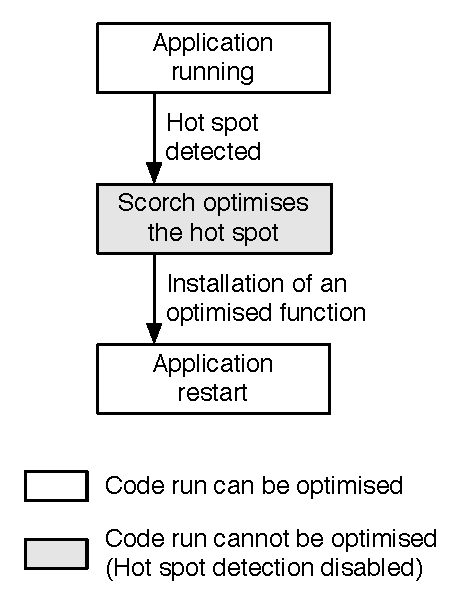
\includegraphics[width=0.4\linewidth]{Disabling}
        \caption{Hot spot detection disabled in critical mode.}
        \label{fig:Disabling}
    \end{center}
\end{figure}

Figure \ref{fig:Disabling} shows the first solution. The application code can be optimised by Scorch, but Scorch cannot optimise its own code when run in critical mode as hot spot detection is disabled. When Scorch is started in background mode, then hot spots are detected (as in any application) and the optimiser code can get optimised.

%1st sol work and good enough 
This first solution is implemented, stable and works fine. Multiple benchmarks run with significant speed-up over the normal VM (This will be detailed in Chapter \ref{chap:validation}). In general, in our production VM, simplicity is really important to keep the code base relatively easy to maintain. For each added complexity in the VM we evaluate if the complexity is worth the benefit. This first solution is very valuable to us because it is fairly simple to understand and to maintain. Hence, the optimising JIT may move to production with this design. The next section discusses alternative solutions, which are more complex but allow, at least partially, the optimiser to optimise its own code when run in critical mode.

\subsection{Discussion and advanced solutions}

%but cannot optimise itself in critical mode
The first solution is working but has one major drawback: Scorch optimiser cannot optimise itself in critical mode. Indeed, hot spots detected inside the optimiser in critical mode are completely ignored and the corresponding profiling counters are reset. If the optimiser attempts to optimise code later, it may get confused by some counter values which were reset (basic block usage is incorrectly inferred in this case, in the worst case, a branch may be speculated as unused whereas it is frequently used). 

\paragraph{Decay strategy.} Instead of resetting entirely the counters, we could implement a decay strategy, by for example dividing the current counter values by two. We did not go in this direction because the counters are currently encoded in 16 bits while the hot spot threshold is set to the maximum value. Due to the 16 bits encoding limitation, not completely resetting the counters leads to the detection of many hot spots, repeatedly, without any optimisation happening slowing down the optimiser at start-up. Further analysis in this direction are required to conclude anything.

%the postpone pb while in critical mode - Saving current stack impossible
\paragraph{Partial disabling.} \label{par:PartialDisabing} Another naive approach is to postpone the optimisation of to background mode when the infinite recursion issue happens in critical mode. In our design, it is quite difficult to do so. Indeed, when the VM call-back starts the optimiser, it provides only a reification of the current stack as detailled in Section \ref{ss:stackSearch}. The optimiser then needs to search the stack to select a function to optimise, and only then it can add a function to optimise to the background compilation queue. 

The stack is modified upon execution and may reference a very large graph of objects, so it is very difficult to save it efficiently for the optimiser to search it later in the background green thread. In addition, as discussed in Section \ref{ss:stackSearch}, there is no obvious cheap heuristic to figure out what function is the best to optimise based on the current stack. 

It is however possible, once the optimiser has found what function to optimise, to add it to the background compilation queue. Therefore, we believe that instead of disabling the entire optimiser while it is running in critical mode, we could instead disable it only during the stack searching phase in critical mode and postpone the optimisation to the background green thread instead if the function to optimise has already been found. This way, only hot spots detected during the stack search would be ignored, while the rest of the optimiser would be optimised at the next idle pause. As the stack search phase represents less than 1\% of the optimiser execution time, this approach looks very interesting.

Figure \ref{fig:PartialDisabling} shows the solution proposed. When a hot spot is detected, Scorch is activated on a stack to optimise and starts by searching a function to optimise. During this phasis, the optimiser is disabled to avoid the infinite recursion issue. Once the function to optimise is found, Scorch optimises it. During this phasis, if a hot spot is detected, the optimiser searches a function to optimise and directly adds it to the background compilation queue. Once the function is optimised, the optimised v-function is installed and the application can resume.

\begin{figure}[h!]
    \begin{center}
        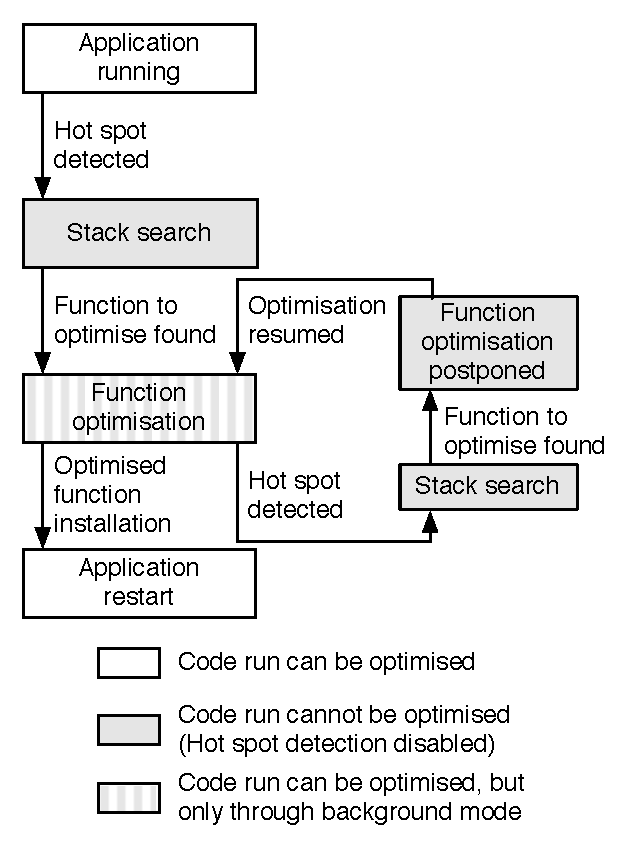
\includegraphics[width=0.55\linewidth]{PartialDisabling}
        \caption{Partial disabling of the optimiser.}
        \label{fig:PartialDisabling}
    \end{center}
\end{figure}

\paragraph{Ahead-of-time optimisation.} 
Alternatively, we could consider optimising the Scorch optimiser code ahead-of-time.

As the Sista architecture allows to persist optimised code (this is discussed in details in the following chapter), the optimiser code could be optimised ahead of time. The optimised optimiser code would be shipped to production, and no runtime optimisation would happen on the optimiser code in production.

To generate the optimised code ahead-of-time, one way is to preheat the optimiser through warm-up runs. For example, the optimiser can be given a list of well-chosen functions to optimise. This way, all hot spots inside the optimiser would be detected ahead of time and optimised. 

Alternatively, the optimiser's code could be optimised statically by calling itself on its own code, using types inferred from a static type inferencer instead of types inferred from the runtime. This solution has a significant cost in our case as we have to implement and maintain a library to infer types.

%\subsection{Dependencies and optimisations} 

% from 1 old part
%Rephrase -  solution does not forbig Scorch to use optimise libs

% maybe only one sentence ? -> be careful about dependencies
%The first constraint to note when programming Scorch, which may be obvious to the Kernel programmer, is that Scorch cannot depends on any framework or library but the Kernel and Core libraries. Each framework or library in the system relies on the execution engine to perform its code. Scorch is part of the execution engine. Hence, if Scorch relies on an external library and that someone modifies the library, the execution engine may not be stable any more and the runtime completely crashes. In fact, all the Kernel code and Core librairies have similar constraints, they cannot rely on anything to keep the system modular. 

%While writting Scorch, we needed a tool to compress the deoptimisation metadata generated aside from the optimised code. We wanted to use the standard Pharo serializer, Fuel (CITE), but we were not able to do it or further modification on Fuel would break the execution engine.

%In the end, we limited the dependencies of Scorch to the Pharo Kernel and the core collections (exactly: Set, OrderedCollection, Array, ByteArray and Dictionary in addition to the kernel). Any change on one of this dependency may require to change something in Scorch to keep the system running.

%\subsection{Debugging and runtime modification}

%Should I talk about that at all ? I was thinking over a restricted compiling to C but maybe we don't care.

%Maybe rewrite so that formally does not work but in practice it does.

%As any Smalltalk program, it is possible to modify the optimiser while it is running, for example in the debugger. If the modifications leads to incorrect optimiser behavior, then the runtime may crash. To avoid crashes, it may be wise to disable the optimiser while editing it. In practice, this feature is used only by the optimiser implementors. It is very useful to debug the optimiser to understand specific bugs or compiler decisions. With careful understanding of the infrastructure, it is possible in practice to debug the optimiser while it is running and modify its code. The optimiser is set by default to catch all exceptions, failing the optimisation of a specific v-function if an exception was raised. Hence, if the code modification triggers a compile-time exception, the system shall not crash. Unfortunately, in some cases, the optimiser may have silent errors, generating incorrect code without raising exceptions and completely crashing the system.

%The only part of Scorch that cannot really be edited is the deoptimisation metadata generation. Indeed, deoptimisation metadata is also used by the deoptimiser which, as detailled in the following section, has stronger constraints on its code. If one modifies the deoptimisation metadata generated, the deoptimiser may not be able to deoptimise correctly optimised code any more, leading to crashes.

%%%%%%%%%%%%%%%%%%%%%%%%%%%%%%%%%%%%%%%%%%%%%%%%%%%%%%%%%%%%%%%%%%%%%%%%%%%%%%%%%%%%%%%%%%%%%%%%%%%%%%%%%%%%%%%%%%%%%%%%%%%%%

%KEEP WRITING FROM HERE

\section{Scorch deoptimiser}
\label{sec:deoptRec}

The deoptimiser can be activated in multiple situations. If an optimisation time assumption is invalid at runtime, a deoptimisation guard fails and Cogit triggers a call-back to deoptimise the stack. In addition, multiple development tools in the language, such as the debugging tools, may call the deoptimiser to introspect the stack.

\subsection{Infinite recursion issue}

% repeat problem for deopt
As Scorch deoptimiser is written in Smalltalk, its code base may get optimised. If one of the optimisation-time speculation is incorrect at runtime, the optimised frame requires the deoptimiser to restore the non-optimised stack frames to continue the execution of the program. 

In the case where the deoptimiser functions are optimised, the deoptimiser may call itself on one of its own frame to be able to continue deoptimising code. If at each deoptimisation the deoptimiser calls itself on one of its own frame, the deoptimisation cannot terminate because the deoptimiser needs to call itself again. The application then gets stuck in an infinite loop.

Figure \ref{fig:InfiniteRecursionDeoptPb} shows the problem in the case where the deoptimiser is triggered by a guard failure. On the left, in the normal deoptimisation flow, the application is interrupted when a guard fails. The deoptimiser recreates the unoptimised stack frames from the optimised stack frame and edits the stack. The application can then resume with unoptimised code. On the right, in the infinite recursion issue, the application is also interrupted when a guard fails. However, while the deoptimiser is deoptimising the stack, another guard fails in the deoptimiser code. The deoptimiser then restarts to deoptimise one of its own frame, but another guard fails in its own code. The deoptimiser keeps restarting the deoptimisation of one of its own frame and the application gets stuck in an infinite loop.

\begin{figure}[h!]
    \begin{center}
        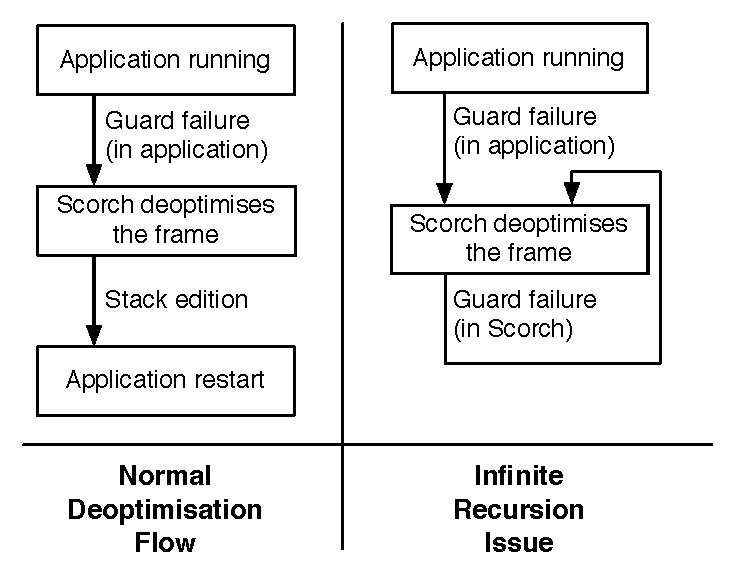
\includegraphics[width=0.65\linewidth]{InfiniteRecursionDeoptPb}
        \caption{Infinite recursion problem during deoptimisation}
        \label{fig:InfiniteRecursionDeoptPb}
    \end{center}
\end{figure}

This problem was solved in the optimiser by disabling it temporarily in specific circumstances. The optimiser could be disabled as the execution could simply fall back to unoptimised code. The deoptimiser cannot however be disabled or any application green thread requiring deoptimisation would not be able to keep executing code. As the deoptimiser cannot be disabled, it is not possible to solve the infinite recursion problem in the same way than the optimiser. 

To solve this infinite recursion problem, we tried to implement two solutions. The first solution, described in Section \ref{sec:recovery}, attempts to restore the runtime in a "recovery mode" when recursive deoptimisation happens. In recovery mode, no optimised function can be used (the runtime relies entirely on the v-function interpreter and the baseline JIT). This solution was used successfully for a subset of the current set of benchmarks. However, this solution was not very good for applications and benchmarks using multiple green threads. We then designed and implemented a second solution, detailled in Section \ref{sec:independentLib}, that is still in use now. The second solution consists in keeping all the deoptimiser code in a library completely independent from the rest of the system that cannot be optimised.

\subsection{Recovery mode}
\label{sec:recovery}

As a first attempt to solve the infinite recursion issue for the deoptimiser, Scorch was modified to keep a recovery copy of each method dictionary where optimised v-functions are installed. The recovery copies include only unoptimised v-functions. We added a global flag, marking if a deoptimisation is in progress. If the deoptimiser is activated while a deoptimisation is in progress (this can be known thanks to the global flag), the deoptimiser falls back to recovery mode. To do so, the deoptimiser uses the primitive \ct{become:} (described in Section \ref{par:become}) to swap all method dictionaries with their recovery copy and disables the optimiser not to optimise anything in the recovery copies. The deoptimiser can then deoptimise the stack without calling itself repeatedly as it now uses only unoptimised functions. Once the stack is deoptimised, the deoptimiser restores the method dictionaries with the optimised v-functions and re-enables the optimiser. 

Figure \ref{fig:InfiniteRecursionDeoptPbRecovery} shows how the recovery mode solves the infinite recursion issue in the deoptimiser. The application is interrupted when a guard fails, and the deoptimiser recreates the unoptimised stack frames from the optimised stack frame. If another guard fails in the deoptimiser code, Scorch falls back to recovery mode, and deoptimises its stack frame using only unoptimised code. Once done, Scorch deactivates the recovery mode to resume the deoptimisation of the application optimised frame. In the worst case, the deoptimiser may switch multiple times to recovery mode to deoptimise the application frame. One the unoptimised stack frames are recreated, the application can resume with non-optimised code.

\begin{figure}[h!]
    \begin{center}
        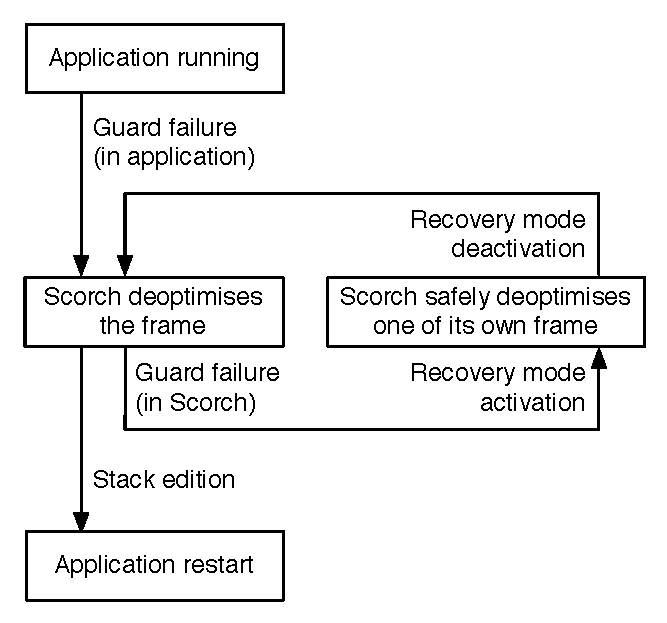
\includegraphics[width=0.6\linewidth]{InfiniteRecursionDeoptPbRecovery}
        \caption{Infinite recursion problem solved with recovery mode}
        \label{fig:InfiniteRecursionDeoptPbRecovery}
    \end{center}
\end{figure}

With this solution, most of the deoptimiser code can be optimised. Indeed, if an infinite recursion happens, Scorch is able to switch to recovery mode and executes correctly the code. Although most of the deoptimiser code can be optimised, not all the code can be. The Smalltalk code executed from the guard failure call-back to the point where recovery mode is activated cannot be optimised. Such code is not protected by the recovery mode and may suffer from the infinite recursion issue. To avoid the problem, we marked a very small list of functions so they cannot be optimised.

\paragraph{Issues.} We were able to run most benchmarks with this solution. However, some benchmarks showed significant slow-down during deoptimisation. Moreover, other benchmarks (the ones using multiple green threads) were crashing. With this solution, we had two major problems. 

The first problem is that switching to recovery mode requires to edit many look-up caches in the VM to use unoptimised functions. Each look-up cache entry referencing an optimised function needs to be edited to refer back to the unoptimised function. Once the deoptimisation in recovery mode is terminated, the caches need to be updated again to reference the optimised functions. Updating all the caches can take a significant amount of time. In addition, in our implementation, the inline caches are directly written in the native code of each n-function. Each update in the native code requires the processor to partially flush its instruction cache. The recovery mode therefore slows down the application for a short while due to the time spent for the VM to update the caches but also to the cpu instruction cache flush and miss (due to the flush).

The second and main problem is that several of our benchmarks use multiple green threads. In this case, the global flag approach to mark if a deoptimisation is in progress does not work as multiple deoptimisations may happen concurrently. In a normal application, when such a problem happens, a developer uses semaphores or other green thread management features present in the language to make the code green thread safe. In the case of Pharo, most of the code related to green thread management and scheduling is written in Pharo itself. Using this code to mark if a deoptimisation is in progress in a process would require it to be marked in the list of functions that cannot be optimised, as this is used in-between the guard failure call-back and the activation of the recovery mode. We did not want to disable optimisations on code present in the semaphores and the process scheduler as such code may be performance critical in some applications. Forbidding the optimisation of such code seemed to be too restrictive. We concluded that this approach could not work for our production environment.

\subsection{Independent library}
\label{sec:independentLib}

As a second solution, we designed the whole deoptimiser as a completely independent Smalltalk library. The deoptimiser may use primitive operations but is not allowed to use any external function. All the deoptimiser classes are marked: their functions do not have profiling counters and the Scorch optimiser is aware that the optimisation of such functions is not allowed. The deoptimiser code is therefore not optimised at runtime, it is running using only the v-function interpreter and the baseline JIT. As the deoptimiser code cannot be optimised and cannot use any external function that could be optimised, the infinite recursion issue cannot happen.

\paragraph{Constraints.} This solution has three main constraints:
\begin{enumerate}
	\item \emph{The deoptimiser code cannot be optimised at runtime.} All the deoptimiser classes are marked not to be optimised at runtime, forbidding the deoptimiser code to reach high performance like the rest of the code. This constraint may be considered as minor as deoptimisation is uncommon. Not optimising the deoptimiser code may therefore not be a problem as the overall time spent in executing its code is very low. In addition, this problem can be partially solved by optimising the deoptimiser code ahead-of-time using Scorch only with optimisations that do not require deoptimisation guards and type information inferred statically. As the library is quite small (500 LoC) and has a very strong invariant (it cannot call any external function), a type inferencer can be easy to implement, very precise and efficient.
	\item \emph{The deoptimiser code needs to be completely independent.} Only primitive operations can be used directly because any external function called may be optimised, potentially leading to the infinite recursion problem. To remove the dependencies to external functions, we analysed what librares the deoptimiser depended on. Most dependencies were very small (for instance accessors to the reification of stack frames) and they could be removed by duplicating a bit of code. However, one dependency was a problem: the deoptimiser uses arrays and dictionaries to deoptimise the stack. Those classes are used in many application so we cannot just forbid to optimise their code base. To solve this issue, we created a minimal array and a minimal dictionary as part of the deoptimiser library that cannot be optimised. The two collections have a separate code base from the classical collection library, which needs to be maintained in parallel to the core collections. As mentioned in the previous paragraph, the overall optimiser code base is very small (500 LoC including the duplicated collections), so we believe it is possible to maintain it without too much effort.
	\item \emph{Work on the deoptimiser is very tedious.} A simple thing such as logging a string in the deoptimiser code for debugging requires to call an external function and may lead to the infinite recursion problem. Understanding and debugging the deoptimiser code is therefore quite difficult.
\end{enumerate}

Although the constraints are important, we were able to run all our benchmarks with this design. We believe we are going to keep this implementation to move to production, at least on the short term.

%%%%%%%%%%%%%%%%%%%%%%%%%%%%%%%%%%%%%%%%%%%%%%%%%%%%%%%%%%%%%%%%%%%%%%%%%%%%%%%%%%%%%%%%%%%%%%%%%%%%%%%%%%%%%%%%%%%%%%%%%%%%%

\section{Related work}
\label{sec:recRelW}

To have an optimising JIT optimising its own code and encounter the infinite recursion problem we discussed in this chapter, the optimising JIT has to be written in one of the languages it can optimise and run in the same runtime than the optimised application. Such an optimising JIT is not common.

Many production VMs are entirely written in a low-level language such as C++~\cite{V8,Webkit15}. The optimising JIT cannot optimise its own code in such VMs. Other VMs such as the ones written with the RPython toolchain ~\cite{Rigo06a} are written in a language that the optimising JIT could optimise, but the production VMs are compiled ahead-of-time to native code, hence the optimising JIT does not optimise its own code at runtime in production. Some VMs are metacircular~\cite{Unga05b,Alp99a}, which means they are entirely written in a language they can run. However, many metacircular VMs, such as Klein~\cite{Unga05b}, do not feature an optimising JIT \footnote{In 2009, Adam Spitz reported some work in the direction of an inlining JIT compiler in Klein on the project web page, but there has been no further news about it since then.}. 

There are two main VMs where the optimising JIT optimises its own code at runtime. On the one hand, there is the Graal compiler~\cite{Oracle13,Dubo13c} which can be used both in the context of the Maxine VM~\cite{Wimm13a} and the Java hotspot VM (CITE). The Graal compiler effectively optimises its own code at runtime as it would optimise the application code. On the other hand, the Jalape\~no VM~\cite{Alp99a}, now called Jikes RVM, features a runtime compiler that can optimise its own code at runtime. 

\subsection{Graal optimising JIT}

The Graal runtime compiler~\cite{Oracle13,Dubo13c} is an optimising JIT written in Java, which is able to optimise its own code at runtime. Graal can be used in different contexts, with different solutions to the infinite recursion problem. Initially, the Graal runtime compiler was designed and implemented as part of the Maxine VM~\cite{Wimm13a}, a metacircular Java VM. Graal was then extracted from Maxine and it can now work on top of the Java hotspot VM (CITE). Graal can be used in two main ways on top of the hotspot VM. On the one hand, it can be used as an alternative optimising JIT, replacing the Java hotspot optimising JIT written in C++. On the other hand, it can be used as a special purpose optimising JIT, optimising only specific libraries or application while the rest of the Java runtime is optimised with hotspot optimising JIT. %VMs built with Truffle~\cite{Wur13a}, a framework allowing to build efficient VMs by simply writting an AST interpreter in Java, are now running using the Java hotspot VM and the Graal compiler as the optimising JIT.

\paragraph{Graal-hotspot architecture.} In our context, the most relevant use-case is when the Graal compiler is used as an alternative optimising JIT on top of the Java hotspot VM. The interpreter and baseline JIT tiers are in this case present in Java hotspot VM, written in a low level language (C++) and compiled ahead-of-time to native code. This is very similar to our design, where the Pharo interpreter and baseline JIT are also compiled ahead-of-time to native code. The optimising JIT are in both cases written in the language run by the VM (Graal in Java and Scorch in Smalltalk), they can optimise their own code and they need to interface with the existing VM to trigger runtime compilation and to install optimised code.

In the Graal-hotspot runtime, when a hotspot is detected, code in the hotspot VM (written in C++) searches the stack for a function to optimise. Once the function is chosen, Hotspot adds it to a thread-safe compilation queue. The Graal compiler is run in different native threads concurrently to the application native threads. Graal takes functions to optimise from the compilation queue, generates concurrently optimised n-function and hands them over to the hotspot VM for installation. The optimised n-functions handed by Graal to hotspot respect the Graal Java native interface~\cite{Grim13a}. They include deoptimisation metadata that the hot spot VM is able to understand. When dynamic deoptimisation happens, code written in the hotspot VM (in C++) is responsible for the deoptimisation of the stack using the metadata handed at installation time.

In our work, Scorch optimiser is able to optimise its own code according to different constraints. The stack search code can be optimised only if the a hot spot is detected while the optimiser is running in background mode. The code responsible for the optimisation of a function can be optimised only indirectly through the background mode. Scorch deoptimiser code cannot be optimised at all. 

\paragraph{Comparison between the architectures.}Table \ref{tbl:comparison} sumarizes the similarities and the differences between the architectures. We call \emph{the base VM} the core elements of the VM excluding the optimising JIT: the interpreter, the baseline JIT and the GC. We then distinguish three parts in the optimising JIT:
\begin{enumerate}
	\item \emph{The stack search:} responsible to find a function to optimise based on a stack with a hot spot.
	\item \emph{The optimisation of a function:} responsible to generate an optimised function based on a non-optimised function and runtime information. This is by far the largest and most complex part of the optimising JIT.
	\item \emph{The deoptimisation of a frame:} responsible to recreate non-optimised stack frames from an optimised frame. 
\end{enumerate}
In both architectures, the base VM is optimised and compiled ahead-of-time (AOT) to executable code. The stack search code is also optimised and compiled ahead-of-time in the case of the Graal-hotspot architecture, while it is running in the same runtime as the application in the case of Scorch. The stack search code can be optimised in Scorch is the hot spot in its code is detected while Scorch is running in background mode. The code responsible to generate the optimised function is in both case running in the same runtime than the application optimised. In the case of Graal-hotspot, the code can be optimised the same way than the application code. In the case of Sista, the optimisation of the function is postponed to the background compilation queue. Lastly, the code responsible for the deoptimisation of a frame is optimised and compiled ahead-of-time in the case of the Graal-hotspot architecture, while it is running in the same runtime than the application in the case of Sista, but cannot be optimised at runtime.

\begin{table}
  \caption{Comparison between the Sista and the Graal-hotspot architectures}
  \vspace{0.1cm}
  \centering
  \begin{tabular}{c||c|c}
    \toprule
    & Sista & Graal-hotspot \\
    \midrule
    \midrule
	Base & Compiled and & Compiled and \\
	VM & optimised AOT & optimised AOT \\
    \midrule
	Stack & Application runtime, optimised & Compiled and \\
	Search & at runtime if hotspot detected & optimised AOT \\
	 & in background mode & \\
    \midrule
	Optimisation & Application runtime, optimised & Application runtime,\\
	of a & at runtime through & optimised at runtime \\
	Function & the background mode & unconditionnally \\
    \midrule
	Deoptimisation & Application runtime, & Compiled and \\
	of a Frame & not optimised at runtime & optimised AOT \\
	\bottomrule
  \end{tabular}
  \label{tbl:comparison}
\end{table}

\paragraph{Notable differences.}Having the stack search and deoptimisation code in Smalltalk, even with constraints, allow us to change part of the design such as the deoptimisation metadata without having to recompile the VM. This is an advantage in our context, as we want Smalltalk developer to be able contribute to the project without having to recompile the VM or look into low-level details. It can however be seen as a draw-back as the constraints, decreases the performance of the deoptimisation of stack frames and the start-up performance of the stack search.

The other difference is with the optimisation of a function. In Sista, Scorch needs to postpone the optimisation to background mode while the Graal-hotspot architecture allows to optimise the function like any application function. Our constraints comes from the fact that Pharo is currently single-threaded. In Graal-hotspot, the optimisation of a function is done in a concurrent native thread. This allows to avoid having a critical and a background mode, as well as allowing the optimising JIT to optimise this part of the code without any constraints. The solution of Graal-hotspot is therefore better, but it could not be implemented in our context.

\subsection{Jikes RVM}

Jikes RVM~\cite{Alp99a,Arn00} optimising runtime compiler is written entirely in Java and can optimise Java code, including its own code. However, it is not currently able to use runtime information to direct its optimisations and do not generate deoptimisation guards~\footnote{"The provided AOS [Adaptive Optimisation System] models do not support Feedback-Directed Optimizations" http://www.jikesrvm.org/ProjectStatus/}, so it is not that relevant in our context. 

The runtime compiler uses however an interesting technique~\cite{Arn00} to choose what function to optimise. Instead of profiling counters, Jikes RVM uses an external sampling profiling native thread. Based on the profiling samples, the profiling thread detect what function should be optimised and adds it to a thread-safe compilation queue. The optimising runtime compiler can then start other native threads which take functions to optimise from the compilation queue, optimise and install them. With this technique, the functions to optimise are chosen entirely concurrently. The application is not interrupted, at any time, to search the stack for a function to optimise or to detect a hot spot. This technique therefore allows to write the hot spot detection in the same runtime than the application optimised, while it can still be optimised the same way than the application run. We did not investigate in this direction because our VM is currently single threaded.

%%%%%%%%%%%%%%%%%%%%%%%%%%%%%%%%%%%%%%%%%%%%%%%%%%%%%%%%%%%%%%%%%%%%%%%%%%%%%%%%%%%%%%%%%%%%%%%%%%%%%%%%%%%%%%%%%%%%%%%%%%%%%

\section*{Conclusion}

In this chapter we discussed the infinite recursion issue. If a hot spot is detected inside the optimiser code, the optimiser may call itself indefinitely to try to optimise it. The deoptimiser has a similar issue when it needs to deoptimise its own code. The problem exists because the optimiser and the deoptimiser are implemented in Smalltalk and are running in the same runtime and the same native thread than the application they optimise and deoptimise respectively. The main issue is related to infinite recursion.

The optimiser solves this issue by disabling itself when it runs in critical mode (when it interrupts temporarily the application green thread to perform the optimisation). %The optimiser cannot optimise itself directly while running in critical mode, it can only optimise the  application, which may include libraries used both by the application and the optimiser itself. For functions taking a long time to optimise, the optimiser cannot stop the application for too long or the application becomes unresponsive, hence it postpone the optimisation to a background compilation queue where functions are optimised when the application is in idle. When performing optimisations in the background, the optimiser can optimise itself entirely.
The deoptimiser has to solve the problem differently as it cannot be disabled temporarily or Smalltalk code cannot be executed any more. The deoptimiser avoids the problem by being written using a small number of classes, independent from the rest of the system, that cannot be optimised nor call any external function.

The next chapter explains how the runtime state is persisted across multiple VM start-ups, including the running green threads and the optimised functions.

\ifx\wholebook\relax\else
    \end{document}
\fi